\documentclass[tikz,border=5pt]{standalone}
\usepackage{amsmath}
\begin{document}
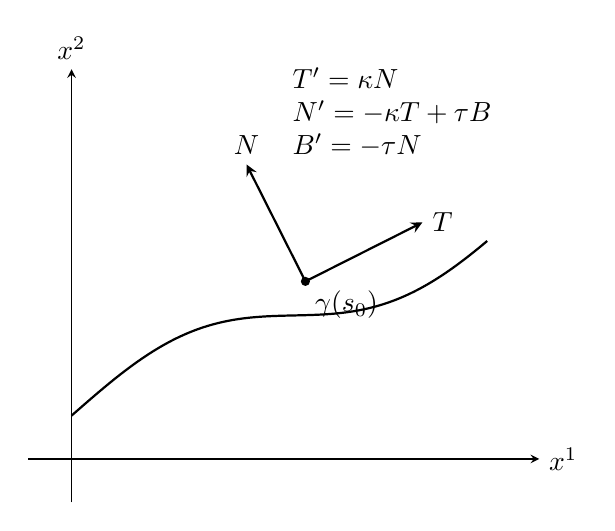
\begin{tikzpicture}[>=stealth,scale=1.1]
  \draw[->] (-0.5,0)--(5.4,0) node[right] {$x^1$};
  \draw[->] (0,-0.5)--(0,4.5) node[above] {$x^2$};
  \draw[thick,domain=0:4.8,samples=120] plot (\x,{0.5+0.45*\x+0.35*sin(70*\x)});
  \coordinate (P) at (2.7,2.05);
  \fill (P) circle (1.5pt) node[below right] {$\gamma(s_0)$};
  \draw[->,thick] (P)--++(1.35,0.68) node[right] {$T$};
  \draw[->,thick] (P)--++(-0.68,1.35) node[above] {$N$};
  \node[align=left] at (3.7,4.0)
  {$T'=\kappa N$\\$N'=-\kappa T+\tau B$\\$B'=-\tau N$};
\end{tikzpicture}
\end{document}
